\begin{quotation}
\ldots
\end{quotation}

\noindent {\em This chapter was derived from a document written by Adam Ferrari and later updated by Alan Batson, Mike Lack, Anita
Jones, and Aaron Bloomfield}

\section{Introduction}

This small guide, in combination with the material covered in the
class lectures on assembly language programming, should provide enough
information to do the assembly language labs for this class. In this
guide, we describe the basics of 32-bit x86 assembly language
programming, covering a small but useful subset of the available
instructions and assembler directives. However, real x86 programming
is a large and extremely complex universe, much of which is beyond the
useful scope of this class. For example, there exists real (albeit
older) x86 code running in the world was written using the 16-bit
subset of the x86 instruction set. Using the 16-bit programming model
can be quite complex~-- it has a segmented memory model, more
restrictions on register usage, and so on. In this guide we'll
restrict our attention to the more modern aspects of 32-bit x86
programming, and delve into the instruction set only in enough detail
to get a basic feel for programming x86 compatible chips at the
hardware level.

\section{Registers}

Modern (i.e., 386 and beyond) x86 processors have eight 32-bit general
purpose registers, as depicted in
Figure~\ref{x86-register-diagram.fig}. The register names are mostly
historical in nature. For example, EAX used to be called the
``accumulator'' since it was used by a number of arithmetic
operations, and ECX was known as the ``counter'' since it was used to
hold a loop index. Whereas most of the registers have lost their
special purposes in the modern instruction set, by convention, two are
reserved for special purposes~-- the stack pointer (ESP) and the base
pointer (EBP).

\begin{figure}[h]
\begin{center}
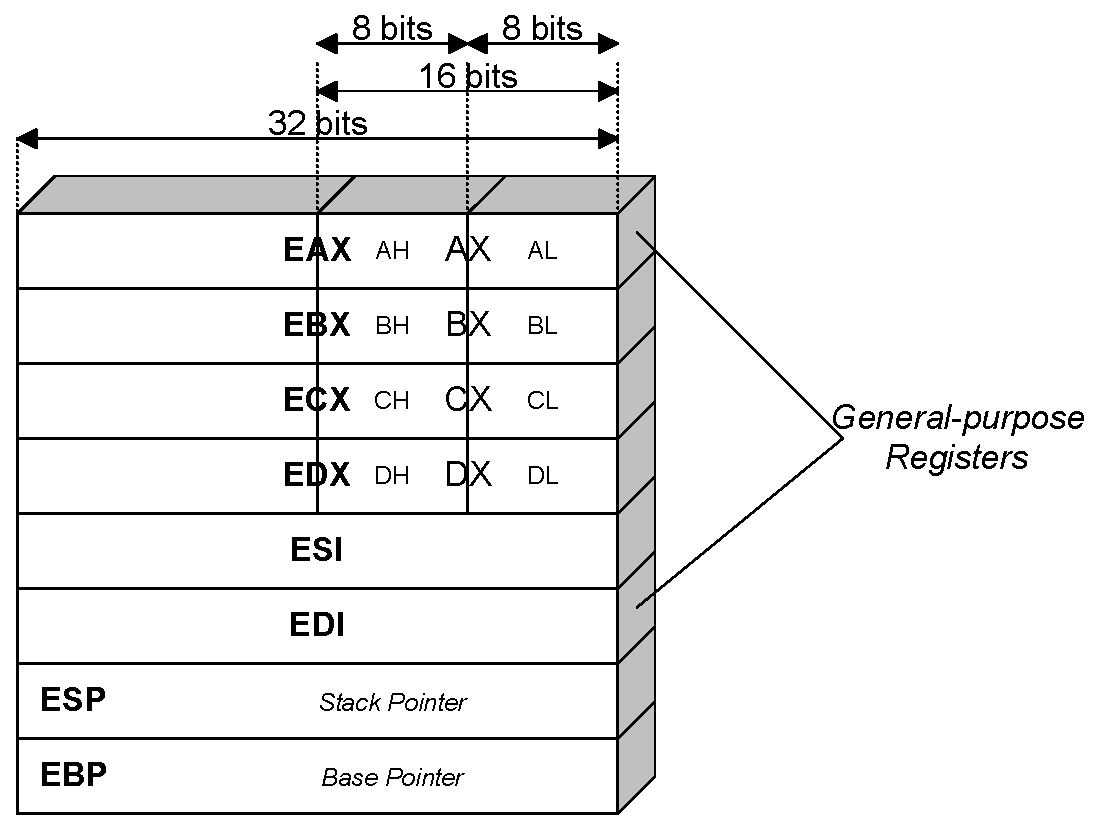
\includegraphics[width=4in]{x86-32bit/x86-register-diagram.pdf}
\end{center}
\caption{The x86 register set}
\label{x86-register-diagram.fig}
\end{figure}

In some cases, namely EAX, EBX, ECX, and EDX, subsections of the
registers may be used.  For example, the least significant 2 bytes of
EAX can be treated as a 16-bit register called AX.  The least
significant byte of AX can be used as a single 8-bit register called
AL, while the most significant byte of AX can be used as a single
8-bit register called AH. It is important to realize that these names
refer to the same physical register. When a two-byte quantity is
placed into DX, the update affects the value of EDX (in particular,
the least significant 16 bits of EDX). These ``sub-registers''
are mainly hold-overs from older, 16-bit versions of the instruction
set. However, they are sometimes convenient when dealing with data
that are smaller than 32-bits (e.g., 1-byte ASCII characters).

When referring to registers in assembly language, the names are not
case-sensitive. For example, the names EAX and eax refer to the same
register.

\section{Memory and Addressing Modes}

\subsection{Declaring Static Data Regions}

You can declare static data regions (analogous to global variables) in
x86 assembly using special assembler directives for this purpose.
Data declarations should be preceded by the .DATA directive. Following
this directive, the directives DB, DW, and DD can be used to declare
one, two, and four byte data locations, respectively. Declared
locations can be labeled with names for later reference - this is
similar to declaring variables by name, but abides by some lower level
rules. For example, locations declared in sequence will be located in
memory next to one another.  Some example declarations are depicted in
Listing~\ref{x86-declaring-memory-regions.lst}.

\begin{figure}[h]
\lstinputlisting[caption=Declaring x86 memory regions,label={x86-declaring-memory-regions.lst},backgroundcolor=\color{white},frame=trBL,linewidth=7in,xleftmargin=0in,language={[x86masm]Assembler}]{x86-32bit/code/memory-regions.s}
\end{figure}

The last example in Listing~\ref{x86-declaring-memory-regions.lst}
illustrates the declaration of an array.  Unlike in high level
languages where arrays can have many dimensions and are accessed by
indices, arrays in assembly language are simply a number of cells
located contiguously in memory. Two other common methods used for
declaring arrays of data are the TIMES directive and the use of string
literals. The TIMES directive tells the assembler to duplicate an
expression a given number of times. For example, the statement ``TIMES
4 DB 2'' is equivalent to ``2, 2, 2, 2''. Some examples of declaring
arrays are depicted in Listing~\ref{x86-declaring-arrays.lst}.

\begin{figure}[h]
\lstinputlisting[caption=Declaring x86 arrays in memory,label={x86-declaring-arrays.lst},backgroundcolor=\color{white},frame=trBL,linewidth=7in,xleftmargin=0in,language={[x86masm]Assembler}]{x86-32bit/code/declaring-arrays.s}
\end{figure}

\subsection{Addressing Memory}
\label{addressing-memory.sec}

Modern x86-compatible processors are capable of addressing up to
$2^{32}$ bytes of memory; that is, memory addresses are 32-bits wide.
For example, in Listings~\ref{x86-declaring-memory-regions.lst} and
\ref{x86-declaring-arrays.lst}, where we used labels to refer to memory
regions, these labels are actually replaced by the assembler with
32-bit quantities that specify addresses in memory. In addition to
supporting referring to memory regions by labels (i.e. constant
values), the x86 provides a flexible scheme for computing and
referring to memory addresses:

{\bf x86 Addressing Mode Rule}~-- Up to two of the 32-bit registers
and a 32-bit signed constant can be added together to compute a memory
address. One of the registers can be optionally pre-multiplied by 2,
4, or 8.

To see this memory addressing rule in action, we'll look at some
example mov instructions.  As we'll see later in
Section~\ref{data-movement-instructions.sec}, the {\tt mov} instruction
moves data between registers and memory.  This instruction has two
operands~-- the first is the destination (where we're moving data {\em
  to}) and the second specifies the source (where we're getting the
data {\em from}). Some examples of mov instructions using address
computations that obey the above rule are shown in
Listing~\ref{x86-valid-addressing-modes.lst}.

\begin{figure}[h]
\lstinputlisting[caption={Valid x86 addressing modes},label={x86-valid-addressing-modes.lst},backgroundcolor=\color{white},frame=trBL,linewidth=7in,xleftmargin=0in,language={[x86masm]Assembler}]{x86-32bit/code/valid-addressing-modes.s}
\end{figure}

Some examples of incorrect address calculations are shown in Listing~\ref{x86-invalid-addressing-modes.lst}.

\begin{figure}[h]
\lstinputlisting[caption={Invalid x86 addressing modes},label={x86-invalid-addressing-modes.lst},backgroundcolor=\color{white},frame=trBL,linewidth=7in,xleftmargin=0in,language={[x86masm]Assembler}]{x86-32bit/code/invalid-addressing-modes.s}
\end{figure}


\subsection{Size Directives}

In general, the intended size of the of the data item at a given memory address can be inferred
from the assembly code instruction in which it is referenced. For example, in all of the above
instructions, the size of the memory regions could be inferred from the size of the register operand~-- when we were loading a 32-bit register, the assembler could infer that the region of memory
we were referring to was 4 bytes wide. When we were storing the value of a one byte register to
memory, the assembler could infer that we wanted the address to refer to a single byte in memory.
However, in some cases the size of a referred-to memory region is ambiguous. Consider the instruction {\tt mov [ebx], 2}.


Should this instruction move the value 2 into the single byte at
address EBX? Perhaps it should move the 32-bit integer representation
of 2 into the 4-bytes starting at address EBX. Since either is a valid
possible interpretation, the assembler must be explicitly directed as
to which is correct.  The size directives {\tt BYTE PTR}, {\tt WORD
  PTR}, and {\tt DWORD PTR} serve this purpose. For examples, see
Listing~\ref{x86-size-directives.lst}.

\begin{figure}[h]
\lstinputlisting[caption={x86 size directive usage},label={x86-size-directives.lst},backgroundcolor=\color{white},frame=trBL,linewidth=7in,xleftmargin=0in,language={[x86masm]Assembler}]{x86-32bit/code/size-directives.s}
\end{figure}


\section{Instructions}

Machine instructions generally fall into three categories: data movement, arithmetic/logic,
and control-flow. In this section, we will look at important examples of x86 instructions from
each category. This section should not be considered an exhaustive list of x86 instructions, but
rather a useful subset.

In this section, we will use the following notation:

\begin{itemlist}
\item $<$reg32$>$ - means any 32-bit register described in Section 2, for example, ESI.
\item $<$reg16$>$ - means any 16-bit register described in Section 2, for example, BX.
\item $<$reg8$>$ - means any 8-bit register described in Section 2, for example AL.
\item $<$reg$>$ - means any of the above.
\item $<$mem$>$ - will refer to a memory address, as described in Section~\ref{addressing-memory.sec}, for example {\tt [EAX]}, or
{\tt [var+4]}, or {\tt DWORD PTR [EAX+EBX]}.
\item $<$con32$>$ - means any 32-bit constant.
\item $<$con16$>$ - means any 16-bit constant.
\item $<$con8$>$ - means any 8-bit constant.
\item $<$con$>$ - means any of the above sized constants.
\end{itemlist}

\subsection{Data Movement Instructions}
\label{data-movement-instructions.sec}

\asminstructionsummary{mov}
{mov $<$reg$>$,$<$reg$>$\newline mov $<$reg$>$,$<$mem$>$\newline mov $<$mem$>$,$<$reg$>$\newline mov $<$reg$>$,$<$const$>$\newline mov $<$mem$>$,$<$const$>$}
{The mov instruction moves the data item referred to by its second
  operand (i.e.  register contents, memory contents, or a constant
  value) into the location referred to by its first operand (i.e. a
  register or memory). While register-to-register moves are possible,
  direct memory-to-memory moves are not. In cases where memory
  transfers are desired, the source memory contents must first be
  loaded into a register, then can be stored to the destination memory
  address.}
{mov eax, ebx \linebreak mov BYTE PTR [var], 5 }
{; transfer ebx to eax\linebreak; store the value 5 into the byte at\linebreak; memory location ``var''}
{2.2in}{3.5in}

\asminstructionsummary{push}
{push $<$reg32$>$\newline push $<$mem$>$\newline push $<$con32$>$}
{The push instruction places its operand onto the top of the hardware supported
stack in memory. Specifically, push first decrements ESP by 4, then places its
operand into the contents of the 32-bit location at address [ESP]. ESP (the stack
pointer) is decremented by push since the x86 stack grows down~-- i.e. the stack
grows from high addresses to lower addresses.}
{push eax\newline push [var]}
{; push the contents of eax onto the stack\newline
; push the 4 bytes at address ``var'' onto stack}
{1in}{4.7in}

\asminstructionsummary{pop}
{pop $<$reg32$>$\newline pop $<$mem$>$}
{The pop instruction removes the 4-byte data element from the top of
  the hardware supported stack into the specified operand (i.e.
  register or memory location). Specifically, pop first moves the 4
  bytes located at memory location [ESP] into the specified register or
  memory location, and then increments SP by 4.}
{pop edi \newline pop [ebx]}
{; pop the top element of the stack into EDI.\newline
; pop the top element of the stack into memory at\newline
; the four bytes starting at location EBX.}
{1in}{4.7in}

\asminstructionsummary{lea}
{lea $<$reg32$>$,$<$mem$>$}
{The lea instruction places the address specified by its second
  operand into the register specified by its first operand. Note, the
  contents of the memory location are not loaded~-- only the effective
  address is computed and placed into the register.  This is useful
  for obtaining a ``pointer'' into a memory region.}
{lea eax, [var]\newline lea edi, [ebx+4*esi]}
{; the address of ``var'' is placed in EAX \newline
; the value EBX+4*ESI is placed in EDI}
{1.85in}{3.85in}

\subsection{Arithmetic and Logic Instructions}

\asminstructionsummary{add, sub}
{add $<$reg$>$,$<$reg$>$ \hspace{0.5in} sub $<$reg$>$,$<$reg$>$ \newline
add $<$reg$>$,$<$mem$>$ \hspace{0.5in} sub $<$reg$>$,$<$mem$>$ \newline
add $<$mem$>$,$<$reg$>$ \hspace{0.5in} sub $<$mem$>$,$<$reg$>$ \newline
add $<$reg$>$,$<$con$>$ \hspace{0.5in} sub $<$reg$>$,$<$con$>$ \newline
add $<$mem$>$,$<$con$>$ \hspace{0.5in} sub $<$mem$>$,$<$con$>$}
{The add instruction adds together its two operands, storing the
  result in its first operand. Similarly, the sub instruction
  subtracts its second operand from its first.  Note, whereas both
  operands may be registers, at most one operand may be a memory
  location.}
{add eax, 10\newline 
sub [var], esi\newline\newline\newline
add BYTE PTR [var], 10}
{; add 10 to the contents of EAX. \newline
; subtract the contents of ESI from \newline
; the 32-bit integer stored at \newline
; memory location ``var''.\newline
; add 10 to the single byte stored\newline
; at memory address ``var''.\newline}
{2.2in}{3.5in}

\asminstructionsummary{inc, dec}
{inc $<$reg$>$ \hspace{0.5in} dec $<$reg$>$\newline
inc $<$mem$>$ \hspace{0.5in} dec $<$mem$>$}
{The inc instruction increments the contents of its operand by one,
  and similarly dec decrements the contents of its operand by one.}
{dec eax \newline inc DWORD PTR [var]}
{; subtract one from the contents of EAX. \newline
; add one to the 32-bit integer stored at \newline
; memory location ``var''.}
{1.8in}{3.9in}

\asminstructionsummary{imul}
{imul $<$reg32$>$,$<$reg32$>$\newline
imul $<$reg32$>$,$<$mem$>$\newline
imul $<$reg32$>$,$<$reg32$>$,$<$con$>$\newline
imul $<$reg32$>$,$<$mem$>$,$<$con$>$}
{The imul instruction has two basic formats: two-operand (first two
syntax listings above) and three-operand (last two syntax listings
above).  The two-operand form multiplies its two operands together and
stores the result in the first operand. The result (i.e., first)
operand must be a register.  The three operand form multiplies its
second and third operands together and stores the result in its first
operand. Again, the result operand must be a register.  Furthermore,
the third operand is restricted to being a constant value.}
{imul eax, [var]\newline\newline\newline
imul esi, edi, 25}
{; multiply the contents of EAX by the \newline
; 32-bit contents of the memory location \newline
; ``var''. Store the result in EAX.\newline
; multiply the contents of EDI by 25. \newline
; Store the result in ESI.}
{1.8in}{3.9in}

\asminstructionsummary{idiv}
{idiv $<$reg32$>$\newline
idiv $<$mem$>$}
{The idiv instruction is used to divide the contents of the 64 bit
  integer EDX:EAX (constructed by viewing EDX as the most significant
  four bytes and EAX as the least significant four bytes) by the
  specified operand value. The quotient result of the division is
  stored into EAX, while the remainder is placed in EDX. This
  instruction must be used with care. Before executing the
  instruction, the appropriate value to be divided must be placed into
  EDX and EAX. Clearly, this value is overwritten when the idiv
  instruction is executed.}
{idiv ebx \newline\newline\newline idiv DWORD PTR [var]}
{; divide the contents of EDX:EAX by the \newline
; contents of EBX. Place the quotient \newline
; in EAX and the remainder in EDX.\newline
; same as above, but divide by the \newline
; 32-bit value stored at memory \newline
; location ``var''.}
{1.9in}{3.8in}

\asminstructionsummary{and, or, xor}
{and $<$reg$>$,$<$reg$>$ \hspace{0.25in} or $<$reg$>$,$<$reg$>$ \hspace{0.25in} xor $<$reg$>$,$<$reg$>$ \newline
and $<$reg$>$,$<$mem$>$ \hspace{0.25in} or $<$reg$>$,$<$mem$>$ \hspace{0.25in} xor $<$reg$>$,$<$mem$>$ \newline
and $<$mem$>$,$<$reg$>$ \hspace{0.25in} or $<$mem$>$,$<$reg$>$ \hspace{0.25in} xor $<$mem$>$,$<$reg$>$ \newline
and $<$reg$>$,$<$con$>$ \hspace{0.25in} or $<$reg$>$,$<$con$>$ \hspace{0.25in} xor $<$reg$>$,$<$con$>$ \newline
and $<$mem$>$,$<$con$>$ \hspace{0.25in} or $<$mem$>$,$<$con$>$ \hspace{0.25in} xor $<$mem$>$,$<$con$>$}
{These instructions perform the specified logical operation (logical
bitwise and, or, and exclusive or, respectively) on their operands,
placing the result in the first operand location.}
{and eax, 0fH \newline xor edx, edx}
{; clear all but the last 4 bits of EAX. \newline ; set the contents of EDX to zero.}
{1.7in}{4in}

\asminstructionsummary{not}
{not $<$reg$>$ \newline not $<$mem$>$}
{Performs the logical negation of the operand contents (i.e., flips all bit values).}
{not BYTE PTR [var]}
{; negate all bits in the byte at the \newline ; memory location ``var''.}
{1.7in}{4in}

\asminstructionsummary{neg}
{neg $<$reg$>$ \newline neg $<$mem$>$}
{Performs the arithmetic (i.e., two's complement) negation of the operand contents.}
{neg eax \newline neg [var]}
{; negate the contents of EAX. \newline ; negate the contests of ``var''}
{1.4in}{4.3in}

\asminstructionsummary{shl, shr}
{shl $<$reg$>$,$<$con8$>$ \hspace{0.5in} shr $<$reg$>$,$<$con8$>$\newline
shl $<$mem$>$,$<$con8$>$ \hspace{0.5in} shr $<$mem$>$,$<$con8$>$\newline
shl $<$reg$>$,cl \hspace{0.92in} shr $<$reg$>$,cl\newline
shl $<$mem$>$,cl \hspace{0.92in} shr $<$mem$>$,cl}
{These instructions shift the bits in their first operand's contents
  left and right ({\tt shl} and {\tt shr}, respectively), padding the
  resulting empty bit positions with zeros. The shifted operand can be
  shifted up to 31 places. The number of bits to shift is specified
  by the second operand, which can be either an 8-bit constant or the
  register CL. In either case, shifts counts of greater then 31 are
  performed modulo 32.}
{shl eax 5 \newline\newline shr [var] 3}{; shift the contents of eax left by 5 bit \newline ; positions \newline ; shift the contents of ``var'' right by 3 \newline ; bit positions}{1.4in}{4.3in}

\subsection{Control Flow Instructions}

In this section, we will refer to labeled locations in the program
text as $<$label$>$. Labels can be inserted anywhere in x86 assembly
code text by entering a label name followed by a colon. For example,
consider the code fragment in Listing~\ref{x86-labeled-code-location.lst}.
The second instruction in this code fragment is labeled ``begin''.
Elsewhere in the code, we can refer to the memory location that this
instruction is located at in memory using the more convenient symbolic
name ``begin'' instead of having to refer to the memory address as an
integer.

\begin{figure}[h]
\lstinputlisting[caption={x86 labeled code location},label={x86-labeled-code-location.lst},backgroundcolor=\color{white},frame=trBL,linewidth=4.75in,xleftmargin=2.25in,language={[x86masm]Assembler}]{x86-32bit/code/labeled-code-location.s}
\end{figure}


\asminstructionsummary{jmp}
{jmp $<$label$>$}
{Transfers program control flow to the instruction at the memory
  location indicated by the operand.}
{jmp begin}{; jumps to the ``begin'' label}
{1.5in}{3.7in}

\asminstructionsummary{jCC}
{je $<$label$>$ ; Jump when equal\newline
jne $<$label$>$ ; Jump when not equal\newline
jz $<$label$>$ ; Jump when last result was zero\newline
jg $<$label$>$ ; Jump when greater than\newline
jge $<$label$>$ ; Jump when greater than or equal to\newline
jl $<$label$>$ ; Jump when less than\newline
jle $<$label$>$ ; Jump when less than or equal to}
{These instructions are conditional jumps that are based on the status
  of a set of {\bf condition codes} that are stored in a special
  register called the {\em machine status word}. The contents of the
  machine status word include information about the last arithmetic
  operation performed. For example, one bit of this word indicates if
  the last result was zero. Another indicates if the last result was
  negative.  Based on these condition codes, a number of conditional
  jumps can be performed. For example, the jz instruction performs a
  jump to the specified operand label if the result of the last
  arithmetic operation (e.g. add, sub, etc.) was zero. Otherwise,
  control proceeds to the next instruction in sequence after the jz.
  These conditional jumps are the underlying support needed to
  implement high-level language features such as ``if'' statements and
  loops (e.g. ``while'' and ``for''). \vspace{6pt}\newline
  A number of the conditional branches are given names that are
  intuitively based on the last operation performed being a special
  compare instruction, cmp (see below).  For example, conditional
  branches such as jle and jne are based on first performing a cmp
  operation on the desired operands.}
{cmp eax, ebx \newline jle done}
{; if the contents of eax are less than or \newline
; equal to the contents of EBX, jump to the \newline
; code location labeled ``done''.}
{1.4in}{4.3in}

\asminstructionsummary{cmp}
{cmp $<$reg$>$,$<$reg$>$\newline
cmp $<$reg$>$,$<$mem$>$\newline
cmp $<$mem$>$,$<$reg$>$\newline
cmp $<$reg$>$,$<$con$>$\newline
cmp $<$mem$>$,$<$con$>$}
{Compares the two specified operands, setting the condition codes in
  the machine status word appropriately. In fact, this instruction is
  equivalent to the sub instruction, except the result of the
  subtraction is discarded.}
{cmp DWORD PTR [var], 10\newline jeq loop}
{; if the 4 bytes stored at memory\newline
; location ``var'' equal the 4-byte\newline
;  integer value 10, then jump to the\newline
; code location labeled loop}
{2.2in}{3.5in}

\asminstructionsummary{call}
{call $<$label$>$}
{This instruction implements a subroutine call that operates in
cooperation with the subroutine return instruction, ret, described
below. This instruction first pushes the current code location onto
the hardware supported stack in memory (see the push instruction for
details), and then performs an unconditional jump to the code location
indicated by the label operand. The added value of this instruction
(as compared to the simple jmp instruction) is that it saves the
location to return to when the subroutine completes.}
{call my\_subroutine}
{; jumps to the ``my\_subroutine'' label, \newline
; pushing the return address onto the \newline
; stack}
{1.8in}{3.9in}

\asminstructionsummary{ret}
{ret}
{In cooperation with the call instruction, the ret instruction
  implements a subroutine return mechanism. This instruction first
  pops a code location off the hardware supported in-memory stack (see
  the pop instruction for details). It then performs an unconditional
  jump to the retrieved code location.}
{ret}{; returns to the address on the top of the stack}
{1in}{4.7in}


\section{Basic Program Structure}
\label{x86-basic-program-structure.sec}

\begin{wrapfigure}{r}{0.37\textwidth}
\lstinputlisting[backgroundcolor=\color{white},frame=trBL,linewidth=2.5in,xleftmargin=0.25in,label={x86-return2.s.lst},language={[x86masm]Assembler},caption={x86 code to return 2}]{x86-32bit/code/return2.s}
\vspace{-0.25in}
\end{wrapfigure}

Given the above repertoire of instructions, you are in a position to
examine the basic skeletal structure of an assembly language
subroutine suitable for linking into C++ code. Unlike C++, which is
often used for the development of complete software systems, assembly
language is most often used in cooperation with other languages such
as Fortran, C, and C++. Commonly, most of a project is implemented in
the more convenient high-level language, and assembly language is used
sparingly to implement extremely low-level hardware interfaces or
performance-critical ``inner loops.'' Thus, in addition to
understanding how to program in assembly language, it is equally
important to understand how to link assembly language code into
high-level language programs.

Before examining the linkage conventions, we must first examine the
basic structure of an assembly language file. To do this, we can
compare a very simple assembly language file to an equivalent C++
file. In Listings~\ref{x86-return2.s.lst} and \ref{x86-return2.cpp.lst} we see
two files, one in C++, the other in x86 assembly. Each file includes a
function (albeit an ugly one) to return the integer value 2.

The top of the assembly file contains two directives that indicate the
instruction set and memory model we will use for all work in this
class (note, there are other possibilities~-- one might use only the
older 80286 instruction set for wider compatibility, for example).

Next, where in the C++ file we find the declaration of the global
variable ``var'', in the assembly file we find the use of the .DATA
and DD directives (described in Section 3.1) to reserve and initialize
a 4-byte (i.e., integer-sized) memory region labeled ``var''.

\begin{wrapfigure}{r}{0.37\textwidth}
\lstinputlisting[backgroundcolor=\color{white},frame=trBL,linewidth=2.5in,xleftmargin=0.25in,label={x86-return2.cpp.lst},language=C++,caption={C++ code to return 2}]{x86-32bit/code/return2.cpp}
\vspace{-0.25in}\end{wrapfigure}

Next in each file, we find the declaration of the function named
returnTwo. In the C++ file we have declared the function to be extern
``C''. This declaration indicates that the C++ compiler should use C
naming conventions when labeling the function returnTwo in the
resulting object file that it produces. In fact, this naming
convention means that the function returnTwo should map to the label
\_returnTwo in the object code. In the assembly code, we have labeled
the beginning of the subroutine \_returnTwo using the PROC directive,
and have declared the label \_returnTwo to be public. Again, the
result of these actions will be that the subroutine will map to the
symbol \_returnTwo in the object code that the assembler generates.

The function bodies are straight-forward. As we will see in more
detail in Section 6, return values for functions are placed into EAX
by convention, hence the instruction to move the contents of ``var''
into EAX in the assembly code.

\begin{wrapfigure}{r}{0.48\textwidth}
\lstinputlisting[backgroundcolor=\color{white},frame=trBL,linewidth=4in,xleftmargin=0.25in,label={x86-calling-return2.cpp.lst},language=C++,caption={Calling returnTwo() from C++}]{x86-32bit/code/calling-return2.cpp}
\vspace{-0.25in}
\end{wrapfigure}

Given these equivalent function definitions, use of either version of
the function is the same.  A sample call to the function returnTwo is
depicted in Listing~\ref{x86-calling-return2.cpp.lst}. This C++ code
could be linked to either definition of the function and would produce
the same results (note, we could not link to both definitions, or the
linker would produce a ``multiply defined symbol'' error. The
mechanics of program linking will be discussed in an associated
document that relates to the specific programming environment that you
will use to assemble and run programs.
